
  Un robot cuenta con un conjunto de sensores y un conjunto de actuadores,
cada uno identificado con un número entero.

  Para especificar el comportamiento de un robot en un programa, se crean
señales a partir de las entradas (sensores), se les aplican funciones
y combinan utilizando los combinadores de FRP, y se mapean señales
a las salidas (actuadores).

  Los combinadores \texttt{lift}, \texttt{lift2} y \texttt{folds},
y las primitivas de entrada/salida \texttt{read}, \texttt{output} se
encuentran dentro del bloque \texttt{do} del programa.

  Con las primitivas de entrada/salida se define cómo se conectan
las señales con sensores y actuadores, y con los combinadores se
define un grafo de señales que especifica el comportamiento del robot.
  
  Para que un programa sea válido, el grafo de señales debe ser acíclico.

  El bloque \texttt{do} permite de manera declarativa expresar las
relaciones entre las señales y que funciones se deben aplicar.

  La máquina virtual que interpreta el programa, será la encargada de
darle valores a las señales y actualizarlas, así como actualizar las
salidas de acuerdo a que señal está conectada a ellas.

  A continuación se presenta el conjunto de primitivas y combinadores.

\subsubsection{Read}
%%read
  Para crear una señal a partir de una entrada, se utiliza la
primitiva \texttt{read}, que asocia la señal a un identificador.

  Asumiendo que un robot tiene un sensor de distancia en la entrada
\texttt{INPUT\_DISTANCE} se puede definir una señal \texttt{distance},
que contendrá la distancia en centímetros para cada instante de tiempo.

\begin{center}
\begin{Verbatim}[frame=single]
distance <- read INPUT_DISTANCE
\end{Verbatim}
\end{center}

El tipo de la primitiva \texttt{read} es:

\begin{center}
  $read :: Int \rightarrow Signal\ a $
\end{center}

\subsubsection{Lift}
%%lift
  Usando la primitiva \texttt{lift} se puede aplicar una función
a la señal, y obtener una nueva señal más compleja resultado de la
aplicación.

  Se puede definir una función \texttt{distanceToSpeed} que de acuerdo
a una distancia, calcula la velocidad apropiada a la que se debe mover
un robot, para detenerse si hay un objeto muy cercano y evitar una colisión.

\begin{center}
\begin{Verbatim}[frame=single]
distanceToSpeed n = if (n < MIN_DIST) then STOP else MAX_SPEED
\end{Verbatim}
\end{center}

%%  La primitiva \texttt{lift} combina una función y un valor
%%dependiente del tiempo, y crea un nuevo valor dependiente
%%del tiempo, es decir, aplica una función que transforma
%%una señal en otra:
%%

  Se puede definir la señal \texttt{speed}, resultado de aplicar la
función \texttt{distanceToSpeed} a la señal \texttt{distance}.

\begin{center}
\begin{Verbatim}[frame=single]
speed <- lift distanceToSpeed distance
\end{Verbatim}
\end{center}

Se puede ver en una línea de tiempo, los valores que toma
cada señal.
\begin{center}
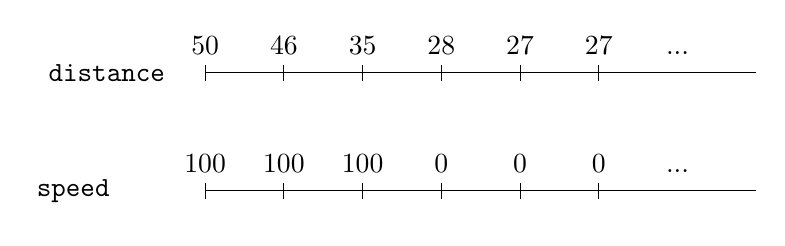
\begin{tikzpicture}
  %draw horizontal line
  \draw (0,1.5) -- (2,1.5);
  \draw (2,1.5) -- (4,1.5);
  \draw (4,1.5) -- (5,1.5);
  \draw (5,1.5) -- (7,1.5);

  %draw vertical lines
  \foreach \x in {0,1,2,3,4,5}
     \draw (\x cm,1.6) -- (\x cm,1.4);

  %draw nodes
  \draw (0,1.5) node[below=3pt] {$  $} node[above=3pt] {$ 50 $};
  \draw (1,1.5) node[below=3pt] {$  $} node[above=3pt] {$ 46 $};
  \draw (2,1.5) node[below=3pt] {$  $} node[above=3pt] {$ 35 $};
  \draw (3,1.5) node[below=3pt] {$  $} node[above=3pt] {$ 28 $};
  \draw (4,1.5) node[below=3pt] {$  $} node[above=3pt] {$ 27 $};
  \draw (5,1.5) node[below=3pt] {$  $} node[above=3pt] {$ 27 $};
  \draw (6,1.5) node[below=3pt] {$  $} node[above=3pt] {$ ... $};
  \draw (0,1.5) node[left=11pt] {\texttt{distance}};

  %draw horizontal line   
  \draw (0,0) -- (2,0);
  \draw (2,0) -- (4,0);
  \draw (4,0) -- (5,0);
  \draw (5,0) -- (7,0);

  %draw vertical lines
  \foreach \x in {0,1,2,3,4,5}
     \draw (\x cm,3pt) -- (\x cm,-3pt);

  %draw nodes
  \draw (0,0) node[below=3pt] {$  $} node[above=3pt] {$ 100 $};
  \draw (1,0) node[below=3pt] {$  $} node[above=3pt] {$ 100 $};
  \draw (2,0) node[below=3pt] {$  $} node[above=3pt] {$ 100 $};
  \draw (3,0) node[below=3pt] {$  $} node[above=3pt] {$ 0 $};
  \draw (4,0) node[below=3pt] {$  $} node[above=3pt] {$ 0 $};
  \draw (5,0) node[below=3pt] {$  $} node[above=3pt] {$ 0 $};
  \draw (6,0) node[below=3pt] {$  $} node[above=3pt] {$ ... $};
  \draw (0,0) node[left=31pt] {\texttt{speed}};
\end{tikzpicture}
\end{center}


El tipo de la primitiva lift es

\begin{center}
  $lift :: (a \rightarrow b) \rightarrow Signal\ a \rightarrow Signal\ b$
\end{center}

\subsubsection{Output}
%%output
  La primitiva \texttt{output} envía a un actuador el valor de una señal.
  Asumiendo que el motor del robot está identificado con el valor entero
\texttt{OUTPUT\_ENGINE}:

\begin{center}
\begin{Verbatim}[frame=single]
output OUTPUT_ENGINE speed
\end{Verbatim}
\end{center}

  El tipo de la primitiva output es

\begin{center}
$output :: Signal\ a \rightarrow Int \rightarrow ()$
\end{center}
 
  En la Figura \ref{fig:example1} se puede ver el ejemplo completo.


\begin{figure}[h!]
\begin{center}
    \caption{Ejemplo completo}
\begin{Verbatim}[frame=single]
INPUT_DISTANCE = 1
OUTPUT_ENGINE = 1

MIN_DIST = 30
MAX_SPEED = 100
STOP = 0

distanceToSpeed n = if (n < MIN_DIST) then STOP else MAX_SPEED

do {
  distance <- read INPUT_DISTANCE,
  speed <- lift distanceToSpeed distance,
  output OUTPUT_ENGINE speed
}
\end{Verbatim}
   \label{fig:example1}
\end{center}
\end{figure}


\subsubsection{Lift2}

  Para combinar más de una señal, se utiliza la función \texttt{lift2}
que recibe dos señales y produce una nueva aplicando una función.

\begin{center}
$lift2 :: (a \rightarrow b \rightarrow c) \rightarrow Signal\ a \rightarrow Signal\ b \rightarrow Signal\ c$
\end{center}

%  Utilizando \texttt{lift2} se pueden definir funciones \texttt{liftN}
%combinándola sucesivas veces, por ejemplo:
%
%\begin{center}
%$lift3 :: (a \rightarrow b \rightarrow c \rightarrow d) \rightarrow Signal\ a \rightarrow Signal\ b \rightarrow Signal\ c \rightarrow Signal\ d$
%$lift3\ f\ sa\ sb\ sc = lift2\ (lift2\ f\ sa\ sb)\ sc$
%\end{center}
%
%% Solved(Marcos): Segun la gramatica del lenguaje no puedo hacer esto.
%% Solved(Guillermo): Además de no tipar, f no se puede aplicar parcialmente
%% para superar esta limitacion, habria que definir tipos mas complejos y/o
%% aceptar currying.
%% Y si lo saco, pasará algo? :D. Quisiera dejarlo fuera del alcance!

\subsubsection{Folds}

  En \frob{} para mantener un valor que dependa de la historia, se utiliza
el combinador \texttt{folds}.

  El mismo es análogo a la operación \texttt{fold} sobre listas, viendo
una señal como una lista de valores en el tiempo, el combinador aplica una
función al valor actual de una señal y a un valor acumulado.
  De ésta manera se puede crear una nueva señal para representar estado.

  Por ejemplo si se asume definida una señal \texttt{button} que tiene
el valor $1$ cuando se apreta un botón y sino el valor $0$, se puede
contar cuántas veces se apretó el botón utilizando el combinador \texttt{folds}
y una función para sumar el valor acumulado y el nuevo.

\begin{center}
\begin{Verbatim}[frame=single]
count <- folds suma 0 button
\end{Verbatim}
\end{center}

Se pueden ver las señales \texttt{button} y \texttt{count} como los
valores en una línea de tiempo:

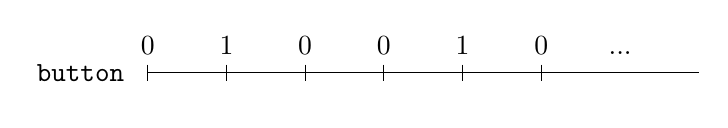
\begin{tikzpicture}
  %draw horizontal line   
  \draw (0,0) -- (2,0);
  \draw (2,0) -- (4,0);
  \draw (4,0) -- (5,0);
  \draw (5,0) -- (7,0);

  %draw vertical lines
  \foreach \x in {0,1,2,3,4,5}
     \draw (\x cm,3pt) -- (\x cm,-3pt);

  %draw nodes
  \draw (0,0) node[below=3pt] {$  $} node[above=3pt] {$ 0 $};
  \draw (1,0) node[below=3pt] {$  $} node[above=3pt] {$ 1 $};
  \draw (2,0) node[below=3pt] {$  $} node[above=3pt] {$ 0 $};
  \draw (3,0) node[below=3pt] {$  $} node[above=3pt] {$ 0 $};
  \draw (4,0) node[below=3pt] {$  $} node[above=3pt] {$ 1 $};
  \draw (5,0) node[below=3pt] {$  $} node[above=3pt] {$ 0 $};
  \draw (6,0) node[below=3pt] {$  $} node[above=3pt] {$ ... $};
  \draw (0,0) node[left=5pt] {\texttt{button}};
\end{tikzpicture}

\begin{tikzpicture}
  %draw horizontal line   
  \draw (0,0) -- (2,0);
  \draw (2,0) -- (4,0);
  \draw (4,0) -- (5,0);
  \draw (5,0) -- (7,0);

  %draw vertical lines
  \foreach \x in {0,1,2,3,4,5}
     \draw (\x cm,3pt) -- (\x cm,-3pt);

  %draw nodes
  \draw (0,0) node[below=3pt] {$  $} node[above=3pt] {$ 0 $};
  \draw (1,0) node[below=3pt] {$  $} node[above=3pt] {$ 1 $};
  \draw (2,0) node[below=3pt] {$  $} node[above=3pt] {$ 1 $};
  \draw (3,0) node[below=3pt] {$  $} node[above=3pt] {$ 1 $};
  \draw (4,0) node[below=3pt] {$  $} node[above=3pt] {$ 2 $};
  \draw (5,0) node[below=3pt] {$  $} node[above=3pt] {$ 2 $};
  \draw (6,0) node[below=3pt] {$  $} node[above=3pt] {$ ... $};
  \draw (0,0) node[left=11pt] {\texttt{count}};
\end{tikzpicture}




El tipo del combinador \texttt{folds} es:

\begin{center}
$folds :: (a \rightarrow b \rightarrow b) \rightarrow b \rightarrow Signal\ a \rightarrow Signal\ b$
\end{center}

%Solved(Marcos): Mostrar un ejemplo completo que combine tod.o.
